\section{Experiment}
\subsection{Entropy of attributes}
Probability distributions, such as normal or uniform distributions, are commonly used to model database' attributes. Much of the popularity of normal distribution can be attributed to the Central Limit Theorem (CLT). The CLT states that, the distribution of the mean which independently has been drawn from the mean of an large number of samples size (N), approaches a normal distribution. The most of data representing human, nature and social sciences often have distributions that are nearly normal. Moreover, algorithms such as Expectation Maximization (EM) can be applied to estimate best likelihood of the observed values to probabilistic models.\\

The entropy is the measure of randomness for an attributes' value set in a database, and entropy is maximized if probability distribution associated with the values is uniform. Intuitively, we compose set of disinformation documents with attributes' value in a way that transfers normal distribution to uniform in database. To exemplify, consider table presented in Figure \ref{attributeEntropy} that presents an attribute with normal and uniform distribution.\\

A normal distribution has a symmetric bell-shape cure and approximately 68\% of data are scattered in the range $[\mu - \sigma, \mu + \sigma]$, and almost 95\% of values lie within $[\mu - 2 \times\sigma, \mu + 2 \times \sigma]$, and about 99.7\% are inside  $[\mu - 3 \times\sigma, \mu + 3 \times \sigma]$. This empirical rule is known as $3\sigma$ rule which discloses critical information about the scatter pattern of a values of data. This leaked information can be exploited by a attacker to guess with high precision.\\ 

We examined a set of databases with different size, containing an attribute with value domain that distributed normally in range $[a,b]$. Then, the comparison of entropy of equivalent attribute with uniform distribution reveals the amount of leaked information from normal distributed data. For instance, the value information from an attribute in the database with 1000 documents in normal distribution is 8.4 bit while in uniform distribution it is 9.97 it means that 1.57 bit of information in normal distribution already leaked. The result is illustrated in Figure \ref{attributeEntropy}. 

%table & chart
\begin{figure}[H]
\hspace*{\fill}%
\begin{minipage}[t]{0.47\linewidth}
\centering
\vspace{0pt}
\begin{tabular}{|c|cc|}
\hline
\multicolumn{1}{|c|}
{\textbf{Db size}} & \multicolumn{2}{c|}
{\textbf{Entropy}}\\
\hline
Document\# & Normal & Uniform\\
\hline \hline
2      &0.5  & 1    \\ 
10     &2.3  & 3.32 \\
$10^2$ &5.4  & 6.64 \\
$10^3$ &8.4  & 9.97 \\
$10^6$ &15.4 & 19.93\\
$10^9$ &21.7 & 29.9 \\
\hline
\end{tabular} 
%\par\vspace{0pt}
\end{minipage}
\begin{minipage}[t]{0.5\textwidth}
\centering
\vspace{0pt}
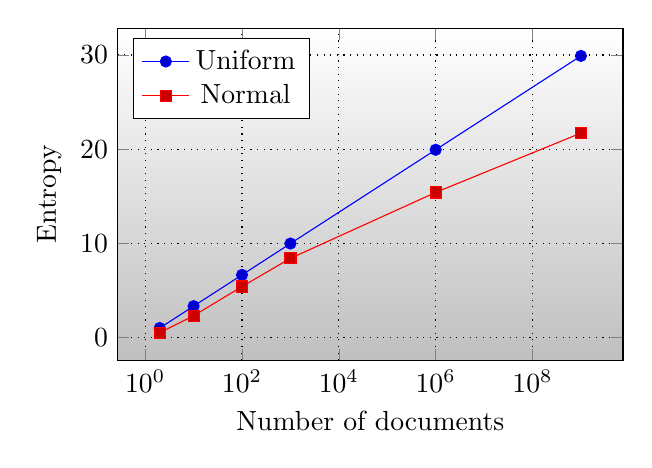
\begin{tikzpicture}
\begin{axis}[legend style={at={(0,0)},anchor=west,at={(axis description cs:1.05,0.45)}},    title={},
xlabel={Number of documents},
xmode = log,        % logarithmic x axis
legend pos=north west,
ylabel={Entropy},
axis background/.style={fill,bottom color=gray!50,top color=white},
grid=major,
height=5.8cm,width=8cm,
grid style={dotted,black}]
\addplot+ coordinates {
(2,1)
(10,3.32)
(100,6.64)
(1000,9.97)
(1000000,19.93)
(1000000000,29.9)
};
\addlegendentry{Uniform}
\addplot+ coordinates {
(2,0.5)
(10,2.3)
(100,5.4)
(1000,8.4)
(1000000,15.4)
(1000000000,21.7)
};
\addlegendentry{Normal}
\end{axis}
\end{tikzpicture}
\end{minipage}%
\caption{Entropy of an attribute in a data set with uniform and normal distribution.}
\label{attributeEntropy}
\end{figure}

%\begin{figure}[H]
%\begin{center}
%\begin{tikzpicture}
%\begin{axis}[legend style={at={(0,0)},anchor=west,at={(axis description cs:1.05,0.45)}},    title={},
%xlabel={Number of documents},
%xmode = log,        % logarithmic x axis
%legend pos=north west,
%ylabel={Entropy},
%axis background/.style={fill,bottom color=gray!50,top color=white},
%grid=major,
%height=6cm,width=8cm,
%grid style={dotted,black}
%]
%\addplot+ coordinates {
%(2,1)
%(10,3.32)
%(100,6.64)
%(1000,9.97)
%(1000000,19.93)
%(1000000000,29.9)
%};
%\addlegendentry{Uniform}
%\addplot+ coordinates {
%(2,0.5)
%(10,2.3)
%(100,5.4)
%(1000,8.4)
%(1000000,16.4)
%(1000000000,23.7)
%};
%\addlegendentry{Normal}
%\end{axis}
%\end{tikzpicture}
%\caption{Entropy of an attribute in sample database with normal and uniform distribution}
%\label{chart:entropyComparison}
%\end{center}
%\end{figure}

\subsection{Query processing time benchmark}
Latency in query execution is the period of time that takes to process the query and return a result set. Indeed, insertion of disinformation documents increases the size of database and it can negatively affect the query execution time. In order to quantify the query latency in cloud DBaaS, an iterative method is employed to evaluate latency of several simple queries on the different databases that are contain specific number of documents. This method, enables us to focus only on a single variable, in this experiment the variable is size of the database. The benchmark initially removes all the existing documents from all databases and repopulated it with the required data set size. Subsequently, a test is performed without index as well as two single index. In all cases, to eliminate cache boost-up, the query caching is disabled. This process is repeated for all the specified database sizes and the measurement for the benchmark with sample queries is displayed in Figure \ref{queryLatencyToSize}a.\\ 

One of the biggest reward of our approach which coming from using the unmodified standard database server is benefit of all database technology’ features such as indexing. Indexing allows to perform more sophisticated search on data such as binary search, that reduces the maximum search time from $O(n)$ to $O(\log n)$ which is magnificent increase in performance. Figure \ref{queryLatencyToSize}b present the improvement of in the same queries' execution time.\\  

\textbf{Result description:} The chart for a simple query on the non-indexed databases demonstrates that query latency steadily increasing with rise of database size. However, the trend of query processing time remains steady with no significant variations with increasing the size of indexed database. The indexed attributes guarantees an insignificant increase in query processing time spatially for the encrypted databases which have the augmented size in comparison with the plaintext non-indexed database.

\input{figures/queryProcessingPerformance.tex}


\subsection{Hash functions performance according to document size }
For preventing active attack on cloud database the eTag algorithm introduced. The eTag constructed based on crypto hash function. We examine the performance of four popular hash functions according the input size. The results is displayed in Figure \ref{fig:hashPerformance}. Considering the performance and security metrics we used Sha1 hash function over others to utilize in eTag algorithm.

%chart
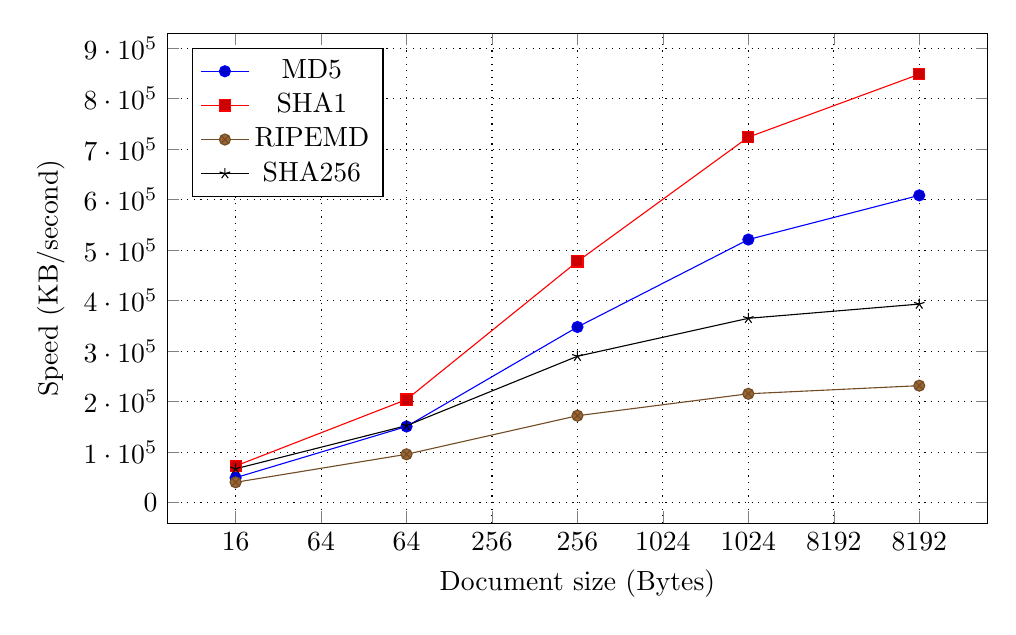
\begin{tikzpicture}
\begin{axis}[legend style={at={(0,0)},anchor=west,at={(axis description cs:1.05,0.45)}},    title={},
ytick={0,100000,200000,300000,400000,500000,600000,700000,800000,900000},
symbolic x coords={16,64,256,1024,8192},
%ytick=data,
xlabel={Document size (Bytes)},
ylabel={Speed (KB/second)},
scaled y ticks=false, 
compat=newest, %Better
legend pos=north west,
%axis background/.style={fill,bottom color=gray!50,top color=white},
grid=major,
height=7.8cm,width=12cm,
grid style={dotted,black}
]
\addplot+ coordinates {
	(16,49292.32)      %16
	(64,150689.13)     %64
	(256,347740.76)    %256
	(1024,520933.03)   %1024
	(8192,608428.03)   %8192
};
\addlegendentry{MD5}
\addplot+ coordinates {
	(16,72490.62)      %16
	(64,204046.66)     %64
	(256,477543.25)    %256
	(1024,723760.47)   %1024
	(8192,848322.56)   %8192
};
\addlegendentry{SHA1}
\addplot+ coordinates {
	(16,40183.96)      %16
	(64,95633.13)      %64
	(256,172034.90)    %256
	(1024,215498.41)   %1024 
	(8192,231541.42)   %8192
};
\addlegendentry{RIPEMD}
\addplot+ coordinates {
	(16,66921.74)      %16
	(64,152366.29)     %64
	(256,289791.49)    %256
	(1024,364940.63)   %1024 
	(8192,393106.77)   %8192
};
\addlegendentry{SHA256}
\end{axis}
\end{tikzpicture}
